% Chapter 2

% Main chapter title
\chapter{Traffic Prediction: Literature Review}

% For referencing the chapter elsewhere, use \ref{Chapter2}
\label{Chapter2}

% This is for the header on each page - perhaps a shortened title
\lhead{Chapter 2. \emph{Traffic Prediction: Literature Review}}

% Quotation
{``There is no way that we can predict the weather six months ahead beyond giving the seasonal
average"}
\begin{flushright}
Stephen Hawking, \textit{Black Holes and Baby Universes} (1993)
\end{flushright}

%---------------------------------------------------------------------------------------------------
%	CONTENT
%---------------------------------------------------------------------------------------------------
\section{Introduction}
%\cite{ahmed1979analysis,van2012short,vlahogianni2004short,vlahogianni2014short,smith1997traffic}
In this chapter we provide a reasonably complete review of existing literature on short term
traffic flow prediction. Research on short term traffic prediction has been going on since 1979,
\citet{ahmed1979analysis}. After more than three decades of research, short term traffic flow
prediction is still an interesting reserch subject for many professionals around the world. The
simplest reseaon being the complex non-linear nature of traffic data and the effects of
non-recurrent events(weather, public events, accidents etc.) on it.  Critical reviews of existing
literature on short term traffic flow have been presented in detail by \citet{smith1997traffic},
\citet{vlahogianni2004short}, \citet{van2012short} and \citet{vlahogianni2014short}. The use of
the phrase 'short term' limits the scope of traffic prediction in terms of the prediction horizon
which usually varies between few seconds to few hours depending upon the approach and application.

The traffic parameter that are predicted can be - flow(number of vehicles per hour), time(minutes
to travel between two points), speed(mean speed in km/hour) and density(number of vehicles per km).

Selecting the right model for short term traffic prediction is a challenging task. A number of
models have been suggested and yet there is no one-fits-all model. The various methods that have
been suggested for short term traffic prediction can be categorised into four groups -
naïve, parametric, non-parametric and hybrid as shown in figure \ref{fig:taxonomyTrafficPrediction}.


\begin{figure}
\centering
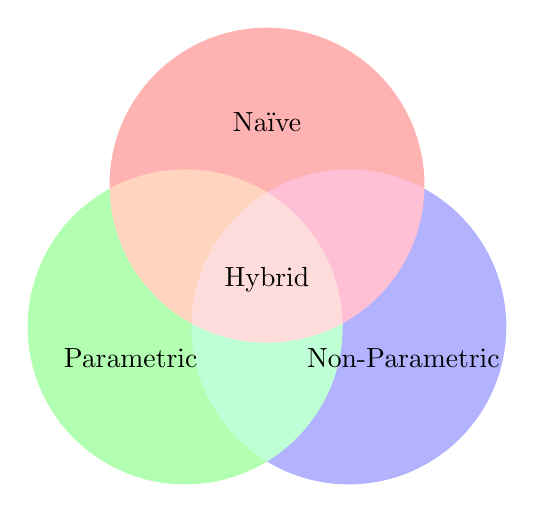
\begin{tikzpicture}
  \begin{scope}[blend group = soft light]
    \fill[red!30!white]   ( 90:1.2) circle (2);
    \fill[green!30!white] (210:1.2) circle (2);
    \fill[blue!30!white]  (330:1.2) circle (2);
  \end{scope}
  \node at (90:2)    {Naïve};
  \node at (210:2)   {Parametric};
  \node at (330:2)   {Non-Parametric};
  \node              {Hybrid};
\end{tikzpicture}
\caption{Methods used for short term traffic prediction} \label{fig:taxonomyTrafficPrediction}
\end{figure}

\section{Naïve methods}
These methods, while called as naive are  sometimes used in practice because of the simplicity
of the method and the ease of implementation. In most cases these methods are used as baselines
for comparison while creating more advances methods. The simplest naive approach in short term
prediction would be to take the last observed value and this involves no computational effort.

Instanteneous Travel Time(ITT) assumes that the traffic conditions will remain constant indefinitly.

Historical averages uses the average of past observed values.

\section{Parametric models}
In parametric models, we estimate the parameters from the training dataset to determine the
function that classifies new unseen data. The number of parameters are fixed. The advantage of
parametric models are that these perform quite well in situations where the large amount of data
is not available. Some of the typical examples of parametric models include Linear and
nonlinear regression, ARIMA models, Kalman filter, Linear SVM etc.

\subsection{Linear and nonlinear regression}
In machine learning and statistical applications, the use of linear models are predominant. These
models are also important in time series domains such as traffic flow prediction. The primary
idea behind the regression is to express the output variable as a linear combination of input
vectors. We can express the linear regression in time series as an ouput influenced by a
collection of inputs, where the inputs could possibly be an independent series

        \begin{equation}
            x_{t} = \beta_{1}z_{t1} + \beta_{2}z_{t2} + ... + \beta_{q}z_{tq} + w_{t}
        \end{equation}

where $ \beta_{1}, \beta_{2},...,\beta_{q} $ are unknown regression coeffiecients and $w_{t}$ is
a random error.

\citet{hogberg1976estimation} used non-liner regression for traffic prediction.

\subsection{ARIMA}
%  Introduction to ARIMA models
% \citet{chen2011short,kumar2015short,min2009short,min2010urban,szeto2009multivariate,
%  van1996combining,williams2001multivariate,williams2003modeling}

ARIMA(Auto Regressive Integrated Moving Average) is a class of parametric regression models. In
this section we will introduce ARIMA and related methods such as exponential smoothing and moving
averages. For an in depth understanding of these models the reader is encouraged to refer to to
~\citet{tong1990non}, ~\citet{brockwell2006introduction} and ~\citet{box2015time}. It is
important to understand that ARIMA modelling works only with stationary time series data. A
stationary time series is one whose properties do not depend on the time it is being observed.
Trends and seasonality affect time series and hence make it non-stationary. Although this seems as a
big restriction, in short term traffic prediction, ARIMA models have been very successful. Two
basic models constituate ARIMA models - AR(autoregressive) and MA(moving average).

The main idea behind autoregressive models is that past values affect the present value, i.e.
$x_{t}$ can be expressed as a function of past p values $ x_{t-1}, x_{t-2},...,x_{t-p} $ , where
p is the number of steps into the past. We can express an autoregressive model of order p as below

        \begin{equation} \label{eq:autoregressive}
          x_{t} = \phi_{1}x_{t-1} + \phi_{2}x_{t-2} + ... + \phi_{p}x_{t-p} + w_{t}
        \end{equation}

where $x_{t}$ is stationary and $\phi_{1}, \phi_{2},..., \phi_{p}$ are constant
parameters that are to be chosen. We have added the term $w_{t}$ as a Guassian white noise with
zero mean and variance $\sigma^{2}_{w}$.

In the MA model, the current value is dependent on the last q one-step forecast errors
$e_{t-1}, e_{t-2},...,e_{t-q}$ and the white noise $w_{t}$. The expression for moving average
is

        \begin{equation} \label{eq:movingaverage}
          x_{t} = -\theta_{1}e_{t-1} - \theta_{2}e_{t-2} - ... - \theta_{q}e_{t-q} + w_{t}
        \end{equation}

$\theta_{1}, \theta_{2},..., \theta_{q}$ are the parameters to be chosen.

Now proceeding to an ARMA(autoregressive moving average) model, we define an ARMA(p,q) model
where the present value $x_{t}$ is dependent on p past recent values and q past recent forecast
errors and a white noise $w_{t}$.

        \begin{equation} \label{eq:arma}
          x_{t} = \phi_{1}x_{t-1} + \phi_{2}x_{t-2} + ... + \phi_{p}x_{t-p} - \theta_{1}e_{t-1}
          - \theta_{2}e_{t-2} - ... - \theta_{q}e_{t-q} + w_{t}
        \end{equation}

When q is 0, the model becomes an autoregressive model of order p, AR(p) and when p is 0 the model
is a moving average of order q, MA(q). We can rewrite \ref{eq:arma} by using the backshift
operator $B^{\alpha}$, which is defined as $B^{\alpha}z_{t} = z_{t-\alpha}$,

        \begin{equation} \label{eq:armarewrite}
          \phi(B)x_{t} = \theta(B)e_{t}
        \end{equation}

where
        \begin{equation}
            \phi(z) = 1 - \phi_{1}z - ... - \phi_{p}z^{p}
        \end{equation}
        \begin{equation}
            \theta(z) = 1 - \theta_{1}z - ... - \theta_{q}z^{q}
        \end{equation}

In practice, most time series data are non-stationary and so several approaches, for instance
by differencing, are taken to make it stationary before applying the ARMA(p,q) model. By
combining differencing with autoregressive and moving average we obtain the ARIMA model defined
as below
        \begin{equation} \label{eq:arima}
          x'_{t} = \phi_{1}x'_{t-1} + \phi_{2}x'_{t-2} + ... + \phi_{p}x'_{t-p} -
          \theta_{1}e_{t-1} - \theta_{2}e_{t-2} - ... - \theta_{q}e_{t-q} + w_{t}
        \end{equation}

where $x'_{t}$ is the differenced series. Formally the model is denotes as ARIMA(p,d,q) where p
is the order of autoregressive part, d is the degree of differencing and q is the order of moving
average. This is also known as a non-seasonal ARIMA model.

The common method used to determine the parameters in an ARIMA(p,d,q) model is known as the
Box-Jenkins approach (\citet{box2015time}) which is three stage procedure. The three stages are
identification, estimation and diagnostic checking. At the identification stage, the values p, d
and q are determined by observing the autocorrelation and partial autocorrelation functions of
the time series and its differences. At the estimation stage, the maximum liklihood estimates are
determined for each model parameter. Finally in the dignostics stage, the residuals are analysed
and model comparisions are done. If the model fits well then the standardised residuals behave as
an i.i.d. with mean zero and variance one.

% Application in traffic forecast
\citet{ahmed1979analysis} used Box-Jenkins method for short-term traffic forecast. The input data
used was 166 sets of time series traffic data collected by freeway traffic surveillance systems in
three locations - Los Angeles, Minneapolis and Detroit. The authors concluded an ARIMA(0,1,3) model
as a resonable fit for the short term prediction task.

\citet{nihan1980use} used the Box-Jenkins technique on monthly data collected on a freeway segment
from 1968 to 1976.

\citet{kumar2015short} used a seasonal ARIMA in a context of limited data for short term traffic 
prediction.

% Conclusions - pros and cons
The major defficiency of tha ARIMA models is that they do not take the extremes into
consideration and focus on the means. This is in contrast to the nature of the traffic data.
ARIMA models are also have the inability to perform will with missing data as pointed out by
\citet{smith1997traffic}.

\subsection{Exponential smoothing}
In exponential smoothing method the forecast is the weighted average of past observations, while
the weights decrease exponentially for older observations. For time series data with no trends
and seasons single exponential smoothing is usually used.


\subsection{Kalman filter}
% \citet{guo2010real,guo2014adaptive,okutani1984dynamic,wang2005real,xie2007short}
\citet{okutani1984dynamic} used Kalman filtering in traffic prediction in an urabn network and
extended it for freeways.

The main advantage of Kalman filtering is the state variable is updated continuously.

\subsection{Other parametric models}

\section{Non-Parametric models}
In nonparamtric models the parameters are not fixed, and vary with the amount of data available.
Usually more data is required for this models than parametric models. The advantage of these models
is that they can model the complex non-linear data better. Some of the widely used non-parametric
models are - k-Nearest Neighbour, Non-parametric regrssion and Neural Networks

\subsection{K-nearest neighbour}
% \citet{lv2009real,myung2011travel,zhang2013improved} \citet{meng2015two}

The basic process of the k-nearest neighbour algorithm is described in figure
\ref{fig:KnnProcessFlow}.

\tikzstyle{block} = [rectangle, draw, text width=5em, text centered, rounded corners,
minimum height=4em]
\tikzstyle{line} = [draw, -latex']
\tikzstyle{cloud} = [draw, ellipse, node distance=4cm, minimum height=3em]

\begin{figure}
\centering
\begin{tikzpicture}[node distance = 3cm, auto]
    % Place nodes
    \node [block] (pp) {Preprocess Data};
    \node [cloud, left of=pp] (hd) {Historical data};
    \node [cloud, right of=pp] (rd) {Real-time data};
    \node [block, below of=pp] (msv) {Match state vector};
    \node [block, below of=msv] (knn) {K nearest neighbour};
    \node [block, left of=knn, node distance=3cm] (prd) {Predictions};
    % Draw edges
    \path [line] (pp) -- (msv);
    \path [line] (msv) -- (knn);
    \path [line] (knn) -- (prd);
    \path [line,dashed] (hd) -- (pp);
    \path [line,dashed] (rd) -- (pp);
\end{tikzpicture}
\caption{K nearest neighbour process flow} \label{fig:KnnProcessFlow}
\end{figure}

\subsection{Fuzzy logic}
% \cite{zhang2008short}

\subsection{Bayesian networks}
% \cite{castillo2008predicting}

\subsection{Neural networks}
% \cite{adeli2001neural,abu2011modeling,bengio1994learning,boto2010wavelet,chan2012neural,
% chan2012optimization,chan2013prediction,chen2001study,dia2001object,dougherty1997short,
% haykin2009neural,hochreiter2001gradient,hodge2014short,hosseini2012short,
% innamaa2005short,ishak2004optimizing,jiang2005dynamic,karlaftis2011statistical,kirby1997should,
% qiu2011bayesian,sun2012network,van2005accurate,vlahogianni2005optimized,
% vlahogianni2007prediction,vlahogianni2013testing,yasdi1999prediction,zheng2006short}
\label{subsec:neuralNetworksTrafficPred}
Artificial Neural Networks(ANN) were mathematical models (\citet{mcculloch1943logical},
\citet{rosenblatt1958perceptron}) designed to  provide a representation of how the human brain
works. It is obvious now that these mathematical models bear little resemblance to the structure
of brain, yet they have been hugely successful. Because they were initially inspired by the
biological brain, the term neural is associated with such kind of mathematical models. A basic
artificial neural network consists of a set of nodes connnected by edges with weights. We can say
that the nodes represent the biological neurons and the edges represent the synapses. The
conections among the nodes can be cyclic or acyclic. The former is known as a feedforward neural
network and the later as a recurrent network. We describe about these neural networks in more
details in chpater \ref{Chapter4}.

Several variations of artificial neural networks have been used in short term traffic prediction.
Some well known examples include - \textit{Multilayer perceptrons, Radial basis function
networks, Kohnen maps} and \textit{Hopfield networks}.


\subsection{Other nonparametric models}

\section{Hybrid Methods}
% \cite{alecsandru2003hybrid,alecsandru2004hybrid,chan2012neural,chen2001study,dimitriou2008adaptive,
% hong2011hybrid,mccrea2010hybrid,wang2013short,xiang2010new,zeng2008short,zhang2014hybrid}


\section{Comparisons}
